\documentclass[11pt]{article}
\usepackage{mathtools}
\usepackage{mdframed}
\usepackage{fullpage}
\usepackage{amsfonts}
\usepackage{tikz}
\usepackage{fancyhdr}
\usepackage{lastpage}
\usepackage{enumitem}
\usepackage{graphicx}

\graphicspath{{coms486/hw3/}}

%edit this for each class
\newcommand\name{John Collin Vincent}
\newcommand\classname{Com S 486}
\newcommand\assignment{Homework 3}


\newcounter{excounter}
\setcounter{excounter}{1}
\newcommand\ques[2]{\vskip 1em  \noindent\textbf{\arabic{excounter}\addtocounter{excounter}{1}.} \emph{#1} \noindent#2}
\newenvironment{question}{\ques{}\begin{quote}}{\end{quote}}
\newenvironment{subquestion}[1]{#1) \begin{quote}}{\end{quote}}

\pagestyle{fancy}
\rfoot{\name, page \thepage/\pageref{LastPage}}
\cfoot{}
\rhead{}
\lhead{}
\renewcommand{\headrulewidth}{0pt}
\renewcommand{\footrulewidth}{0pt}
\DeclarePairedDelimiter\ceil{\lceil}{\rceil}
\DeclarePairedDelimiter\floor{\lfloor}{\rfloor}


\begin{document}

  {\bf \classname \hspace{1cm} \assignment\hfill \name}
  \vskip 2em

  \begin{question}
    \begin{enumerate}[label=\alph*)]
        \item 280
        \item 331
        \item 280, 1234, 2096
        \item 311
        \item \text{}\\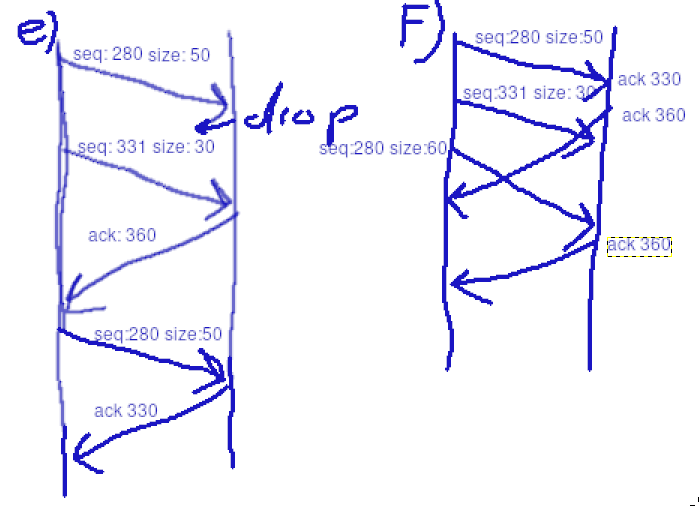
\includegraphics[width=0.7\linewidth]{pic.png}
    \end{enumerate}
  \end{question}

  \begin{question}
    it would take 3 time blocks with any ordering with a possible solution being\\
    $\{x,y,z\},\: \{y,x,null\},\: \{null,null,y\}$\\
    with FIFO ordering you would have to take 4 with a possible solution being \\
    $\{y,null,null\},\: \{x,null,y\},\: \{null,y,z\}, \{null,x,null\}$
  \end{question}

  \clearpage

  \begin{question}
    \begin{subquestion}{a}
        \begin{tabular}{| c | c |}
            \hline
            ip & interface \\ \hline
            240.0.0.0/12 & 0 \\ \hline
            240.8.0.0/16 & 1 \\ \hline
            240.0.0.0/7 & 2 \\ \hline
            242.0.0.0/7 & 2 \\ \hline
            0.0.0.0/0 & 3 \\ \hline
        \end{tabular}
    \end{subquestion}
    \begin{subquestion}{b} 
        3, 2, 2, 1 
    \end{subquestion}
  \end{question}

  \begin{question}
    by adding two more bits to the submask we can get the 4
    different networks. $123.4.56.0/26$, $123.4.56.64/26$, 
    $123.4.56.128/26$, $123.4.56.192/26$. Each network will 
    support 64 host.
  \end{question}

  \begin{question}
    all of the packets will have the same id 166. All but the
    last packet will have the fragflag set to signify there 
    are more packet fragments coming. There will be 4 packets
    of length 800, and the last packet will be length 400. For 5 
    total fragments.
    The offset field will start at 0 and increase by 800 for each
    subsequent packet.
  \end{question}

  \begin{question}
    \begin{align*}
        \frac{3,000,000 + 20x}{1,500} &= x\: packets\\
        \frac{3,000,000}{1,500} &= x - \frac{x}{75}\\
        2000 &= \frac{74x}{75}\\
        \ceil{2000(\frac{75}{74})} &= x\\
        x &= 2,028\: packets
    \end{align*}
  \end{question}

\end{document}
